\section{Preliminaries}
\label{sec:prelim}
A graph $g$ is represented as a five-tuple $g=(V, E, \Sigma_V,\Sigma_E, L)$, where $V(g)$ is the vertex set of $g$, $E(g) \subseteq V(g) \times V(g)$ is the edge set of $g$, $\Sigma_V$ and $\Sigma_E$ are the sets of vertex and edge labels, and $L$ is a label function that maps each node $v\in V(g)$ and each edge $e \in E(g)$ to a label. For unlabelled graph, $\Sigma_V$ and $\Sigma_E$ are $\emptyset$. For a node $v\in V(g)$, we use $id(v)$ to denote its index, $\mathcal{N}(v)$ to denote its neighbours, $d(v)=|\mathcal{N}(v)|$ to denote its degree, $N=|V(g)|$ and  $M=|E(g)|$ to denote its node and edge size, respectively. We use $d_{avg}(g) = \frac{2N}{M}$ and $d_{max}(g) = \max_{v\in V(g)}d_g(v)$ to denote $g$'s average and maximum degree, respectively. A graph g is a \textit{clique} if it is a complete graph. $k\text{-}clique$ is a clique consisting of $k$ nodes. A graph $g$ is a \textit{star} if it is a tree with depth $1$. $k\text{-}star$ is a tree with one root node and $k$ leaf nodes.\\

Given two graphs $g_1$ and $g_2$, $g_1$ is a subgraph of $g_2$, denoted as $g_1 \subseteq g_2$, iff (1) $\forall v\in V(g_1), v\in V(g_2)$ and $L_{g_1}(v)=L_{g_2}(v)$; (2) $\forall (v_i,v_j)\in E(g_1), (v_i,v_j)\in E(g_2)$ and $L_{g_1}((v_i,v_j))=L_{g_2}((v_i,v_j))$.\\

\begin{definition}
\label{def:isomorphism}{\textbf{(Subgraph Isomorphism)}} Given a query graph $q$ and data graph $G$, $q$ is subgraph isomorphic to $G$ iff there exists a subgraph $g\subseteq G$ and a bijection $f: V(q) \rightarrow V(g)$ such that (1) $\forall v \in V(q)$, $L_q(v) = L_{g}(f(v))$; (2) $\forall (v_1, v_2) \in E(q)$, $(f(v_1), f(v_2)) \in E(g)$, and $L_q((v_1, v_2)) = L_{g}((f(v_1), f(v_2)))$. \\

Here, we call a bijection $f$ a \textit{Match}, which can be represented as a tuple $\mathcal{M}$, consisting of data vertices and each data vertex $u_j$ in $\mathcal{M}$ matches the vertex $v_i$ in query graph $u_j \rightarrow f(v_i)$. An \textit{automorphism} is a graph that is isomorphic to itself.
\end{definition}

\stitle{Problem Statement.} Given a query graph $q$ and data graph $G$, \textit{subgraph matching} is to enumerate all subgraphs in $G$ that are isomorphic to $q$.\\

Given a query graph $q$ and data graph $G$, we denote the subgraph matching result set as $R_G(q)$, or $R(q)$ if the context is clear. \\

\begin{example}
\label{ex:subgraph_isomorphism}	
Given an unlabelled query graph $q$ and a data graph $G$ in \reffig{subgraph_isomorphism}, we use symmetry breaking technique\cite{Grochow2007} to assign a partial order for the query graph which avoids duplicated enumerations caused by automorphism. In this example, the partial order of query graph can be $\{v_2 < v_5\}$ . There are two matches of $(v_1, v_2, v_3, v_4, v_5)$, which are $(u_1, u_2, u_3, u_5, u_6)$ and $(u_4, u_3, u_2, u_6, u_5)$. We can check the order constraint for the first match, namely $(u_1, u_2, u_3, u_5, u_6)$. As we have order $v_2 < v_5$, it constraints that we should have $f(v_2) < f(v_5)$, where $u_2 = f(v_2)$, $u_6 = f(v_5)$ and $u_2 < u_6$ satisfies this constraint. For simplicity, we define that for two nodes $u_i, u_j \in V(G)$, $u_i < u_j$ iff $id(u_i) < id(u_j)$. 
\end{example}

\begin{figure}[htb]
  \centering
  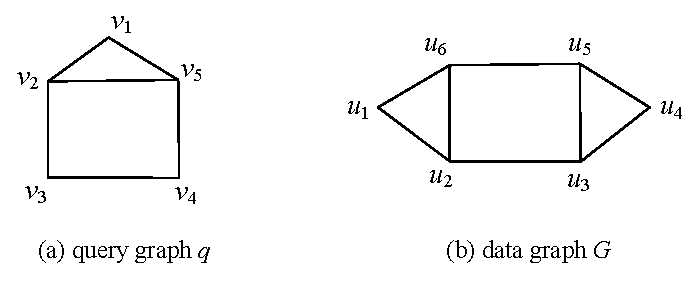
\includegraphics[scale=0.6]{figures/subg.eps}
  \caption{\small{An example of subgraph matching.}}
  \label{fig:subgraph_isomorphism}
\end{figure}

Regarding query vertices as attributes and data vertices as tuples in the relation table, we can naturally express the subgraph join process as joining relations. In \reffig{subgraph_isomorphism}, the edge-by-edge join process can be demonstrated as

\begin{equation}
\label{eq:subgraph_isomorphism}
\small
\begin{aligned}
	R(q) &= R(v_1, v_2) \Join R(v_2, v_3) \Join R(v_3, v_4) \\ 	
	&\Join R(v_4, v_5) \Join R(v_1, v_5) \Join R(v_2, v_5).
\end{aligned}
\end{equation}

\stitle{CliqueJoin.} Generally speaking, the state-of-the-art algorithm \cliquejoin follows the decomposition-and-join framework to do subgraph matching. The main idea of \cliquejoin can be concluded as follows. 

\sstitle{(1) SCP Storage Mechanism.} Considering the SCP storage mechanism for data graph $G$, denoted as $\Phi(G)$, we have $\Phi(G)=\{G_v\ |\ v\in V(G)\}$, $V(G_v)=\{v\} \cup \mathcal{N}(v)$ and $E(G_v)=\{(v,v')\ |\ v'\in \mathcal{N}(v)\}\cup\{(v',v")\ |\ v',v"\in \mathcal{N}(v)\wedge(v',v")\in E(G)\wedge v<v'\wedge v<v"\}$, where $G_v\subseteq G$ is a connected subgraph of $G$ with $v\in V(G_v)$, and $\bigcup_{u\in V(G)}E(G_v)=E(G)$. Each $G_v$ is called the \textit{local graph} of $v$. Suppose the data graph $G$ is maintained in the distributed file system in the form of key-value pairs $(v;G_v)$ for each $v\in V(G)$ according to $\Phi(G)$, a \textit{join unit} is a structure whose matches can be enumerated independently in each local graph $G_v\in \Phi(G)$. For \cliquejoin, the join unit can either be a clique or a star. 

\sstitle{(2) Query Decomposition.} Given a graph storage $\Phi(G)$ and query graph $q$, a query decomposition of $q$ is defined as $D=\{p_0,p_1,\dots,p_t\}$, where each $p_i\in D(0\leq i\leq t)$ is a \textit{join unit} w.r.t. $\Phi(G)$ and $q = \bigcup_{p_i\in D}p_i$. Given the decomposition $D=\{p_0,p_1,\dots,p_t\}$ of $q$, we solve the subgraph enumeration using $t$ rounds of two-way join:

\begin{equation} \label{eq:1}
R(q) = \bowtie_{p_i\in D}R(p_i).
\end{equation}

\sstitle{(3) Optimal Join Plan.} A \textit{join plan} determines an order to solve the above join, which can significantly affect the performance of the algorithm. The join plan is usually presented in a binary tree structure, where the leaf nodes are (the matches of) the join units, the internal nodes are the partial queries. Given a join plan, we compute the join order through a post-order traversal over its binary tree. We denote $P$ as the partial queries set, $P_i$ as the $i$-th partial query whose results are produced in the $i$-th round of the join plan. As a result, a join plan, denoted as $J$, can be uniquely represented as $J = (D, P)$. \cliquejoin utilizes general bushy tree \cite{tree} to represent its join plan. \\

\begin{example}
Figure \ref{fig:tree} shows a join plan for an unlabelled query graph $q$ in the form of a bushy tree. The decomposition of $q$ is $D=\{p_0, p_1, p_2, p_3\}$, and partial query set is $P=\{P_1, P_2, P_3\}$, where $P_3=q$. The first round of join is $P_1 = p_0 \Join p_1$, second round is $P_2=p_2 \Join p_3$, and the final round is $P_3 = P_1 \Join P_2$. In this case, we use triangle ($3$-clique) as the join unit.
\end{example}

\begin{figure}[htb]
  \centering
  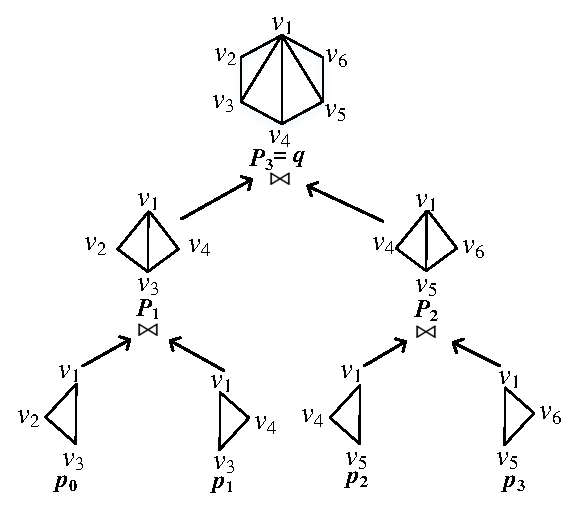
\includegraphics[scale=0.6]{figures/tree.eps}
  \caption{\small{An example of optimal bushy join plan.}}
  \label{fig:tree}
\end{figure}

We denote the set of all possible join plans for query graph $q$ as $\mathcal{S}(q)$. Given a cost function $\mathcal{C}$ defined over $\mathcal{S}$, we say a join plan $\varepsilon$ is \textit{optimal} iff $\mathcal{C}(\varepsilon)$ is minimized. The details of the cost function design can be found in \cite{Lai2016}. However, it is clear that $\mathcal{C}(\varepsilon)$ is positive related to $|R(q)|$.

\sstitle{(4) Matching Result Estimation.} In order to compute the join plan cost  $\mathcal{C}(\varepsilon)$, \cliquejoin needs to estimate $|R(q)|$ for a given query graph $q$. As most of real-life graphs follow \textit{power-law} random distribution\cite{Chung2003}, \cliquejoin estimates $|R_{G_{\text{PR}}}(q)|$ in data graph $G_{\text{PR}}$ generated by power-law model.\\

Considering $q$ is constructed from a single edge by extending one edge at a time in steps. Let $q^{(1)}$ and $q^{(2)}$ be two consecutive queries obtained along the process. More specifically, for some $v\in V(q^{(1)})$ and $v'\in V(q^{(2)})$ such that  $(v,v')\not\in E(q^{(1)})$, $q^{(2)}$ is obtained by adding the edge $(v,v')$ to $q^{1}$. Suppose $f$ is a match of $q^{(1)}$, in principal, we extend $f$ by one more edge to get new matches for $q^{(2)}$. Thus, if the expectation of new matches that can be extended for one certain match of $q^{(1)}$ is $\lambda$, we have:
\begin{equation} \label{eq:r}
|R_{G_{\text{PR}}}(q^{(2)})|=\lambda |R_{G_{\text{PR}}}(q^{(1)})|
\end{equation}

The value of $\lambda$ depends on the edge which extends $q^{(1)}$ to $q^{(2)}$. There are two cases may happen, that is, $v'\not\in V(q^{(1)})$ and $v'\in V(q^{(1)})$. The details of the two cases for computing $\lambda$ and the algorithm of computing $|R_{G_{\text{PR}}}(q)|$ by extending edges can be found in \cite{Lai2016}.

\stitle{Timely Dataflow.} \timely dataflow system is a high performance distributed system. It abstracts the computation model as a dataflow graph. The node in the dataflow graph is responsible for doing computations and the edge is to send data streams to nodes. One node can receive several input streams and produce one output stream. When the dataflow graph for the given computation task is constructed, it will distribute data to each worker in the cluster, and each worker can finish its computation locally. The whole computation task is finished when there is no output stream produced by workers.